\section{Polynomial Hierarchy}
\begin{figure}[h]
    \centering
    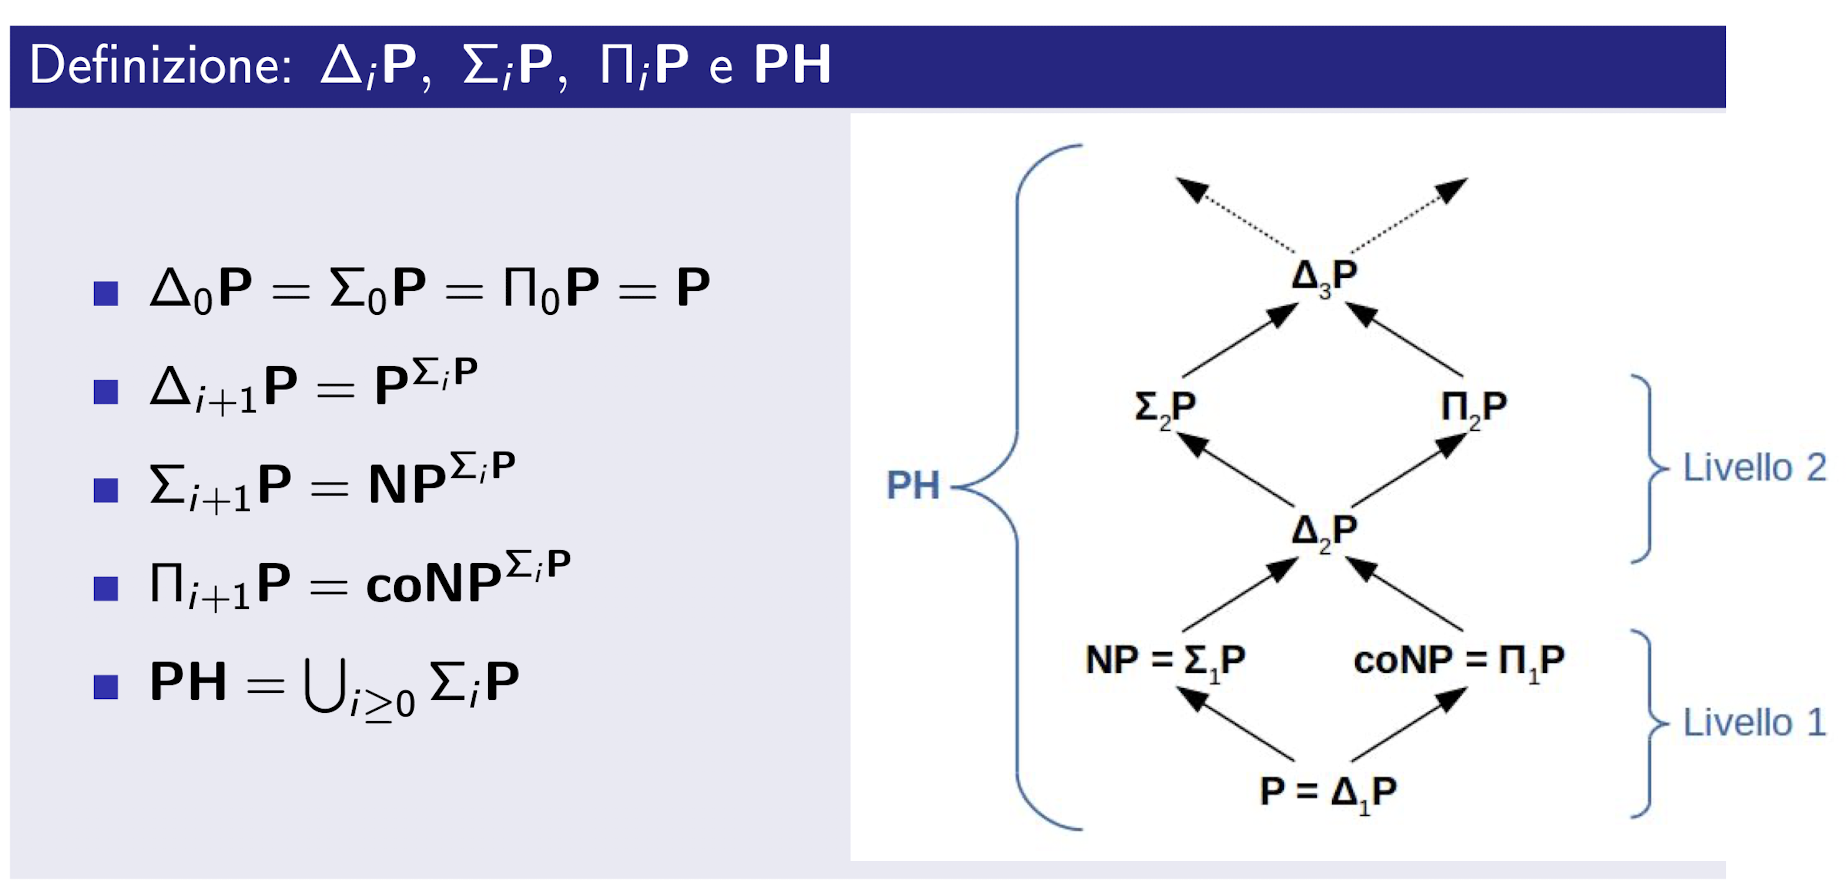
\includegraphics[width=1\textwidth]{img/ph.png}
    \caption{Polynomial Hierarchy}
\end{figure}
Since $\Sigma_0\mathbf{P} = \mathbf{P}$ does not help polynomial-time oracle machines, the first level of this hierarchy makes up our familiar important complexity classes: 
\[
\Delta_1\mathbf{P} = \mathbf{P}, \quad \Sigma_1\mathbf{P} = \mathbf{NP}, \quad \Pi_1\mathbf{P} = \mathbf{coNP}.
\]
The second level starts with the class $\Delta_2\mathbf{P} = \mathbf{P}^{\mathbf{NP}}$ studied in the previous section, and continues with $\Sigma_2\mathbf{P} = \mathbf{NP}^{\mathbf{NP}}$, and its complement $\Pi_2\mathbf{P} = \mathbf{coNP}^{\mathbf{NP}}$. As with the first level, there is every reason to believe that all three classes are distinct. The same holds for the third level, and so on. Naturally, the three classes at each level are related by the same inclusions that we know about $\mathbf{P}$, $\mathbf{NP}$, and $\mathbf{coNP}$. Also, each class at each level includes all classes at previous levels.
\begin{defbox}[Theorem 17.8]
Let $L$ be a language, and $i \geq 1$. $L \in \Sigma_i\mathbf{P}$ if and only if there is a polynomially balanced relation $R$ such that the language $\{x; y : (x, y) \in R\}$ is in $\Pi_{i-1}\mathbf{P}$ and
\[
L = \{ x : \text{there is a } y \text{ such that } (x, y) \in R \}
\]
\end{defbox}
\begin{proof}
    omitted
\end{proof}
\begin{defbox}[Corollary 1]
Let $L$ be a language, and $i \geq 1$. $L \in \Pi_i\mathbf{P}$ if and only if there is a polynomially balanced binary $R$ such that the language $\{x; y : (x, y) \in R\}$ is in $\Sigma_{i-1}\mathbf{P}$ and
\[
L = \left\{ x : \text{ for all } y \text{ with } |y| \leq |x|^k,\, (x, y) \in R \right\}.
\]
\end{defbox}
\begin{proof}
Just recall that $\Pi_i\mathbf{P}$ is precisely $\mathbf{co}\Sigma_i\mathbf{P}$.
\end{proof}
Notice that in the description of $L$ in Corollary 1 we must explicitly state for the universally quantified string $y$ the bound $|y| \leq |x|^k$. Since $R$ is known to be polynomially balanced, this constraint is, in this context, superfluous, and will be omitted. Also, we shall use quantifiers such as $\forall x$ and $\exists y$ in the descriptions of languages such as the one displayed in Corollary 2 below. This will help bring out the elegant mathematical structure of these descriptions, as well as their affinity with logic.

\medskip

In order to get rid of the recursion in the previous Theorem, let us call a relation $R \subseteq (\Sigma^*)^{i+1}$ polynomially balanced if, whenever $(x, y_1, \ldots, y_i) \in R$, we have that $|y_1|, \ldots, |y_i| \leq |x|^k$ for some $k$.
\begin{defbox}[Corollary 2]
Let $L$ be a language, and $i \geq 1$. $L \in \Sigma_i\mathbf{P}$ if and only if there is a polynomially balanced, polynomial-time decidable $(i+1)$-ary relation $R$ such that
\[
L = \left\{ x : \exists y_1 \forall y_2 \exists y_3 \cdots Q y_i \text{ such that } (x, y_1, \ldots, y_i) \in R \right\}
\]
where the $i$th quantifier $Q$ is ``for all'' if $i$ is even, and ``there is'' if $i$ is odd.
\end{defbox}
\begin{proof}
    Repeatedly replace languages in $\Pi_j\mathbf{P}$ or $\Sigma_j\mathbf{P}$ by their certificate forms as in Theorem and its Corollary 1.
\end{proof}
Using these characterizations we can prove the basic fact concerning the polynomial hierarchy: As it is built by patiently adding layer after layer, always using the previous layer as an oracle for defining the next, the resulting structure is extremely fragile and delicate. Any jitter, at any level, has disastrous consequences further up:

\begin{defbox}[Theorem 17.9]
If for some $i \geq 1$ $\Sigma_i\mathbf{P} = \Pi_i\mathbf{P}$, then for all $j > i$ $\Sigma_j\mathbf{P} = \Pi_j\mathbf{P} = \Delta_j\mathbf{P} = \Sigma_i\mathbf{P}$.
\end{defbox}

\begin{proof}
It suffices to show that $\Sigma_i\mathbf{P} = \Pi_i\mathbf{P}$ implies $\Sigma_{i+1}\mathbf{P} = \Sigma_i\mathbf{P}$. So, consider a language $L \in \Sigma_{i+1}\mathbf{P}$. By Theorem 17.8 there is a relation $R$ in $\Pi_i\mathbf{P}$ with 
\[
L = \{x : \text{there is a } y \text{ such that } (x, y) \in R\}.
\]
But since $\Pi_i\mathbf{P} = \Sigma_i\mathbf{P}$, $R$ is in $\Sigma_i\mathbf{P}$. That is, $(x, y) \in R$ if and only if there is a $z$ such that $(x, y, z) \in S$ for some relation $S \in \Pi_{i-1}\mathbf{P}$. Thus $x \in L$ if and only if there is a string $y, z$ such that $(x, y, z) \in S$, where $S \in \Pi_{i-1}\mathbf{P}$. But this means that $L \in \Sigma_i\mathbf{P}$.
\end{proof}

The statements of many results in complexity theory end like that of Theorem 17.9: ``then for all $j > i$ $\Sigma_j\mathbf{P} = \Pi_j\mathbf{P} = \Delta_j\mathbf{P} = \Sigma_i\mathbf{P}$.'' This conclusion is usually abbreviated ``then the polynomial hierarchy collapses to the $i$th level.'' For example:

\begin{defbox}[Corollary]
If $\mathbf{P} = \mathbf{NP}$, or even if $\mathbf{NP} = \mathbf{coNP}$, the polynomial hierarchy collapses to the first level.
\end{defbox}
The last corollary makes one thing abundantly clear: In the absence of a proof that $\mathbf{P} \neq \mathbf{NP}$, there is no hope of proving that the polynomial ``hierarchy'' is indeed a hierarchy of classes each properly containing the next (although, once again, we strongly believe that it is).
The non-monotonic logics were introduced in AI to allow reasoning with incomplete information. The idea is to make plausible assumption that could end up being false in the future. Some examples of non-monotonic logics are Circumscription, Default logic and Answer Set Programming (ASP). The reasoning in the proposition versione of these logics is positioned at the 2° level of the polynomial hierarchy.
\begin{defbox}[The Yale shooting problem]
    If we shoot a turkey with a loaded gun, the turkey is dead. We want to derive that: After reloading the gun and after shooting (in this order), the turkey is dead. The possible actions at time $t$ are: $\text{load}_t, \text{unload}_t, \text{shoot}_t$.
\end{defbox}
Let's model the problem in propositional logic.
\begin{align*}
    &\text{load}_t\to \text{loaded}_{t+1}\\
    &\text{unload}_t\to \neg \text{loaded}_{t+1}\\
    &\text{loaded}_t\land \text{shoot}_t\to \text{dead}_{t+1}\\
    &\text{load}_0 \\
    &\text{shoot}_1 
\end{align*}
Can we conclude that $\text{dead}_2$? 
\\
Yes, we can. It's a logical consequence of the axioms.
\begin{figure}[h]
    \centering
    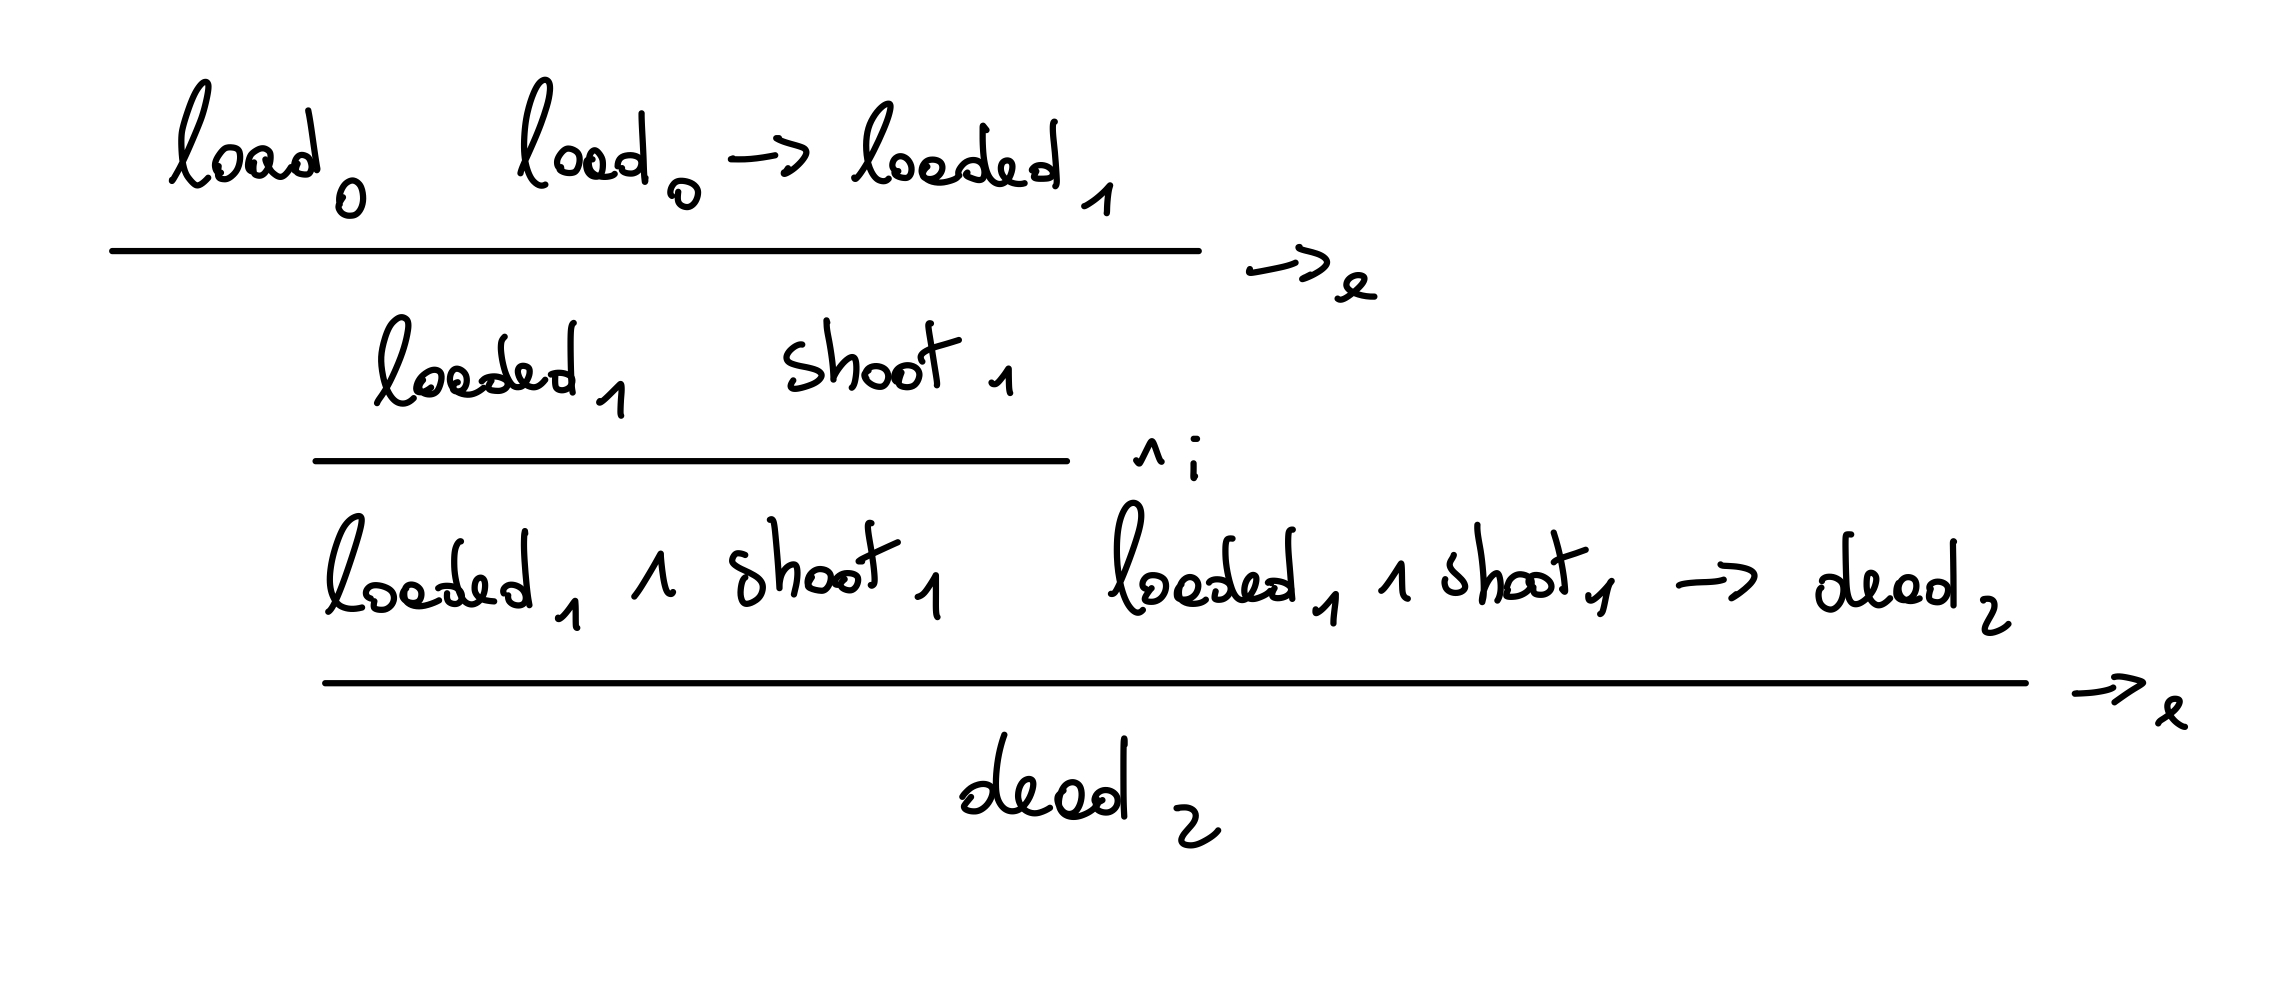
\includegraphics[width=1\textwidth]{img/ysp1.jpeg}
\end{figure}
\\
What about the following situation?
\begin{align*}
    &\text{load}_t\to \text{loaded}_{t+1}\\
    &\text{unload}_t\to \neg \text{loaded}_{t+1}\\
    &\text{loaded}_t\land \text{shoot}_t\to \text{dead}_{t+1}\\
    &\text{load}_0 \\
    &\text{shoot}_2
\end{align*}
Can we conclude $\text{dead}_3$?\\
No, we can't. There is nothing that tells us $\text{loaded}_1 \implies \text{loaded}_2$. That is, nothing tells us that the gun is not unloaded at time 1.\\
Let's try to fix that. 
\begin{align*}
    &\text{load}_t\to \text{loaded}_{t+1}\\
    &\text{unload}_t\to \neg \text{loaded}_{t+1}\\
    &\text{loaded}_t\land \text{shoot}_t\to \text{dead}_{t+1}\\
    &\text{loaded}_t\land\neg\text{unloaded}_t\to \text{loaded}_{t+1}\\
    &\text{load}_0 \\
    &\text{shoot}_2
\end{align*}
Can we conclude $\text{dead}_3$?\\
No, we can't. The gun could be unloaded at time 1. In logic, all that is not specified is not assumed to be false but is not known. So we would need to explicitly say that the gun is not unloaded at time 1. This would be also needed in all successive time steps $[0,t]$. This is not feasible. The commonsense reasoning aims to support a more reasonable representation using non-monotonic logics.\\
Let KB be the set of axioms of the Yale shooting problem. We want to conclude $\text{dead}_3$ from KB assuming that the gun is not unloaded if not specified. In this case the logic is non-monotonic because the set of consequences is not increasing with the addition of new axioms. In the classical logic if KB $\subseteq$ KB' then KB $\vDash$ $\phi$ implies KB' $\vDash$ $\phi$. That is, we cannot invalidate a conclusion by adding new axioms. In the non-monotonic logic, this is not true. We can invalidate a conclusion by adding new axioms.\\
The \textbf{Circumscription} is a non-monotonic logic that allows to reason with incomplete information. The idea is to assume that the world is as simple as possible. In the Yale shooting problem, we can assume that the gun is not unloaded if not specified. This kind of logic is a combination of \textbf{SAT} and a problem of maximization where we want to maximize the number of conclusion that we can draw from the axioms by reducing them. This is what makes the complexity of the problem raise from the 1° level of the polynomial hierarchy to the 2° level.\\
\begin{defbox}[Circumscription]
Let M be the set of propositions that represent abnormal situations, that is the situations that we want to avoid thus we want to make as false as possible. A truth assignment T is preferred (more normal than) to T' iff for every propositional symbol $p\in M$, $T'(p)=\text{false}\implies T(p)=\text{false}$, that is T is at least as normal as T'. In this case we write $T\leq_M T'$. The models of a set of axioms KB (in Circumscription) are the truth assignments T that satisfy KB $(T\vDash KB)$ such that per every T' that satisfies KB, $T'\leq_M T\implies T\le_M T'$. If $\phi$ is true in every model of KB, we write $KB\vDash_M \phi$ and we say that $\phi$ is a logical consequence of KB.\\
\end{defbox}
Now let's see how to use Circumscription to solve the Yale shooting problem. We want to prove that $\text{dead}_3$ is a logical consequence of the axioms. $M={ab_t | t\in\mathbb{N}}$
\begin{align*}
    &\text{load}_t\to \text{loaded}_{t+1}\\
    &\text{unload}_t\to \neg \text{loaded}_{t+1}\\
    &\text{loaded}_t\land \text{shoot}_t\to \text{dead}_{t+1}\\
    &\text{loaded}_t\land\neg\text{ab}_t\to \text{loaded}_{t+1}\\
    &\text{load}_0 \\
    &\text{shoot}_2
\end{align*}
The models here are completely normal: all the $ab_t$ are false. We can derive that $\text{dead}_3$ (KB $\vDash_M$ $\text{dead}_3$).
\begin{figure}[h]
    \centering
    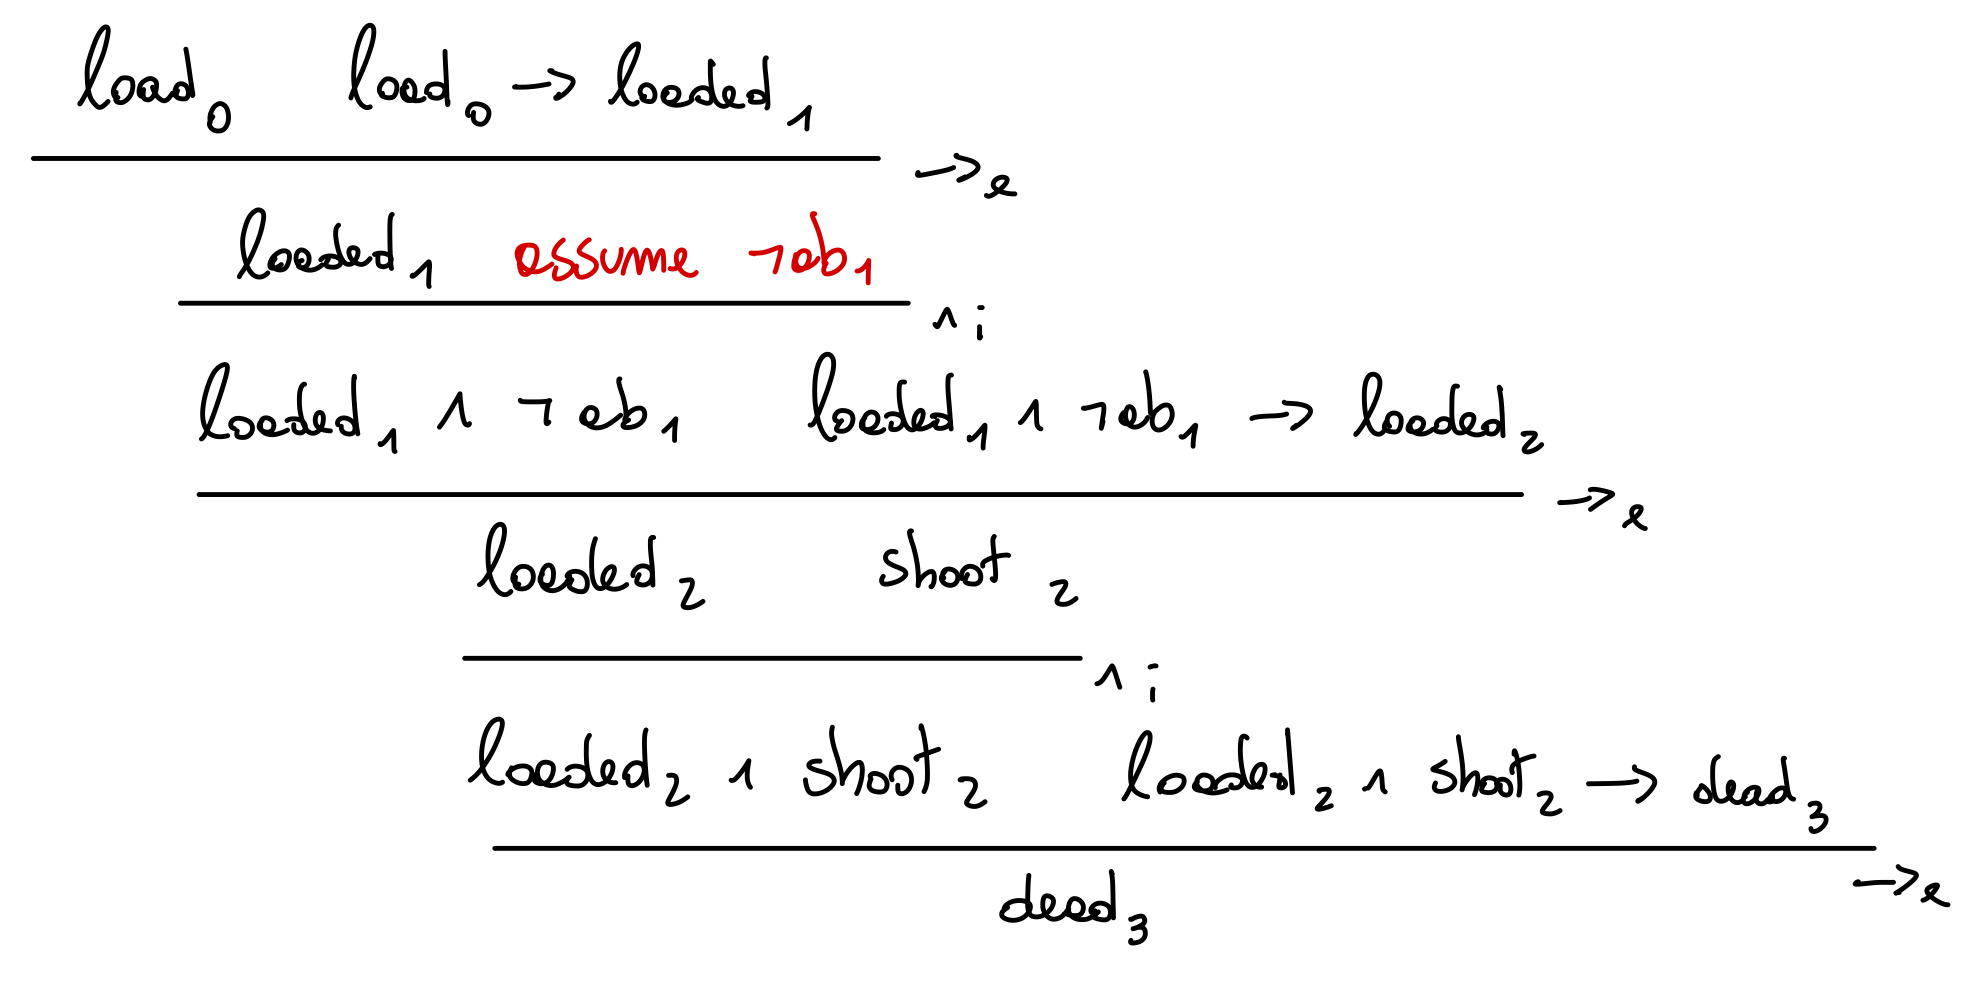
\includegraphics[width=1\textwidth]{img/ysp2.jpeg}
\end{figure}
\\
What about if the gun is unloaded at time 1? 
\begin{align*}
    &\text{load}_t\to \text{loaded}_{t+1}\\
    &\text{unload}_t\to \neg \text{loaded}_{t+1}\\
    &\text{loaded}_t\land \text{shoot}_t\to \text{dead}_{t+1}\\
    &\text{loaded}_t\land\neg\text{ab}_t\to \text{loaded}_{t+1}\\
    &\text{load}_0 \\
    & \textsl{unload}_1 \\
    &\text{shoot}_2
\end{align*}
In this case $\text{unload}_1$ makes $\text{ab}_1$
true in every model of KB to avoid the contradiction $\text{loaded}_2\land \neg\text{loaded}_2$. So we can derive that $\text{dead}_3$ is not a logical consequence of KB.
\begin{figure}[h]
    \centering
    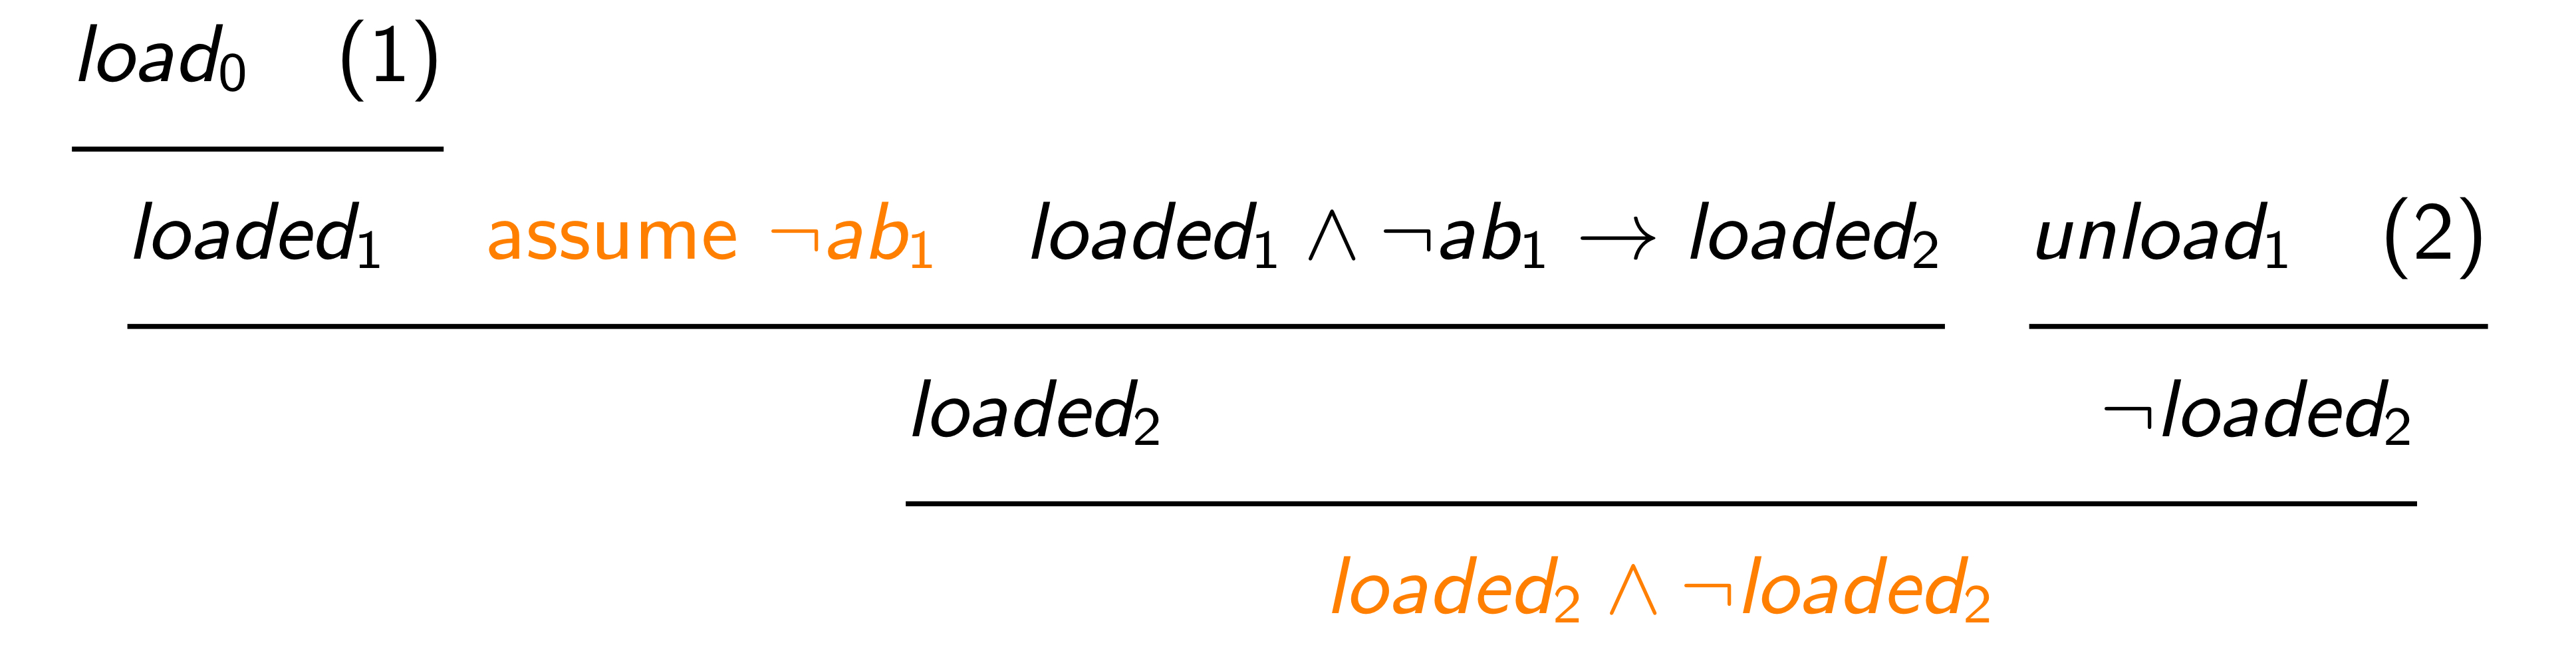
\includegraphics[width=1\textwidth]{img/ysp3.jpeg}
\end{figure}\\
This logic is very flexible, even if we assume $\neg\text{dead}_3$ this makes $\text{ab}_1$ true in every model of KB. So we can derive that $\text{dead}_3$ is not a logical consequence of KB.
\begin{defbox}[Theorem (CIRC SAT and CIRC VALIDITY)]
    Deciding whether a model of KB satisfies $\phi$ is $\Sigma_2\mathbf{P}$-complete.\\
    Deciding whether KB $\vDash_M \phi$ is $\Pi_2\mathbf{P}$-complete.
\end{defbox}
Notice that CIRC SAT $\eqsim$ SAT + minimization of abnormality predicates. As often happens, the complexity of the problem increases when we try to optimize (in this case with minimization) the solution.
The quantified Boolean formulae (QBF) are propositional fragment of the 2° order logic, that is the logic that allows to quantify over the propositional symbols. E.g. $\forall p \exists q.\; \neg p\lor q$ is a QBF. To express the concept of VALIDITY we have something like $\forall p\forall q.\;\neg p\lor p\lor q$. To express satisfiability we have something like $\exists p\exists q.\; p\land q$. To say that a formula in not valid we can say $\forall p\forall q.\; p\lor q$. To say that a formula is not satisfiable we can say $\exists p\exists q.\; p\land \neg p\land q$. In addition to SAT and VALIDITY (1° level) the QBF can express also Circumscription (2° level). For more details refer to the slides. Consequence: The QBF of the form $\exists \vec{x}\forall \vec{y}.\; \phi$ are hard for $\Sigma_2\mathbf{P}$ and the QBF formulae of the form $\forall \vec{x}\exists \vec{y}.\; \phi$ are hard for $\Pi_2\mathbf{P}$. We notice that the number of alternated quantifiers corresponds to the level of the polynomial hierarchy in which the problem is located. Now we give the definition of $QSAT_i$ which is $\Sigma_i\mathbf{P}$-complete.\\
\begin{defbox}[$QSAT_i$]
    Given a QBF with $i$ alternated quantifiers
    \[
\exists p_{1,1} \dots \exists p_{1,n_1} \; \forall p_{2,1} \dots \forall p_{2,n_2} \; \exists p_{3,1} \dots \phi
\]
 more concisely represented as
 \[
\exists \vec{p}_1 \; \forall \vec{p}_2 \; \exists \vec{p}_3 \dots Q \vec{p}_i \; \phi
\]
where $Q$ is $\exists$ if $i$ is odd and $\forall$ if $i$ is even, and where the variables $\vec{p}_1\dots\vec{p}_i$ are all the variables of the formula $\phi$ say if the QBF if true.
\end{defbox}
\begin{defbox}[Theorem]
    $QSAT_i$ is $\Sigma_i\mathbf{P}$-complete.
\end{defbox}
\begin{proof}
omitted
\end{proof}
\begin{defbox}[Theorem]
    CIRC SAT is $\Sigma_2\mathbf{P}$-complete. That is, the problem of deciding whether a formula $\phi$ is true in a model of KB (in the Circumscription logic) is $\Sigma_2\mathbf{P}$-complete.
\end{defbox}
\begin{proof}
    By reduction from $QSAT_2$. Omitted.
\end{proof}
\begin{defbox}
    STRATEGIC COMPANIES is $\Sigma_2\mathbf{P}$-complete.
\end{defbox}
\begin{proof}
    By reduction from $QSAT_2$. Omitted.
\end{proof}
We know that every level of the polynomial hierarchy has same problems that are complete for that level. We don't know if there are problems that are complete for the whole polynomial hierarchy. Is set of all the QBF formulae complete for the whole polynomial hierarchy? Even if seams reasonable to think so the answer is no. Actually it's \textbf{PSPACE}-complete. If we discovered the existence of a problem that is complete for the whole polynomial hierarchy we would have same big consequences.
\subsection{\textcolor{red}{Theorem 17.11}}
\begin{defbox}[\textcolor{red}{Theorem 17.11}]
    If there was a \textbf{PH}-complete problem, then the polynomial hierarchy would collapse to some finite level.
\end{defbox}
\begin{proof}
Suppose that $L$ is \textbf{PH}-complete. Since $L \in \textbf{PH}$, there is an $i \geq 0$ such that $L \in \Sigma_i\mathbf{P}$. But any language $L' \in \Sigma_{i+1}\mathbf{P}$ reduces to $L$. Since all levels of the polynomial hierarchy are closed under reductions, this means that $L' \in \Sigma_i\mathbf{P}$, and hence $\Sigma_i\mathbf{P} = \Sigma_{i+1}\mathbf{P}$.
\end{proof}
\begin{defbox}[Proposition]
    $\textbf{PH}\subseteq\textbf{PSPACE}$
\end{defbox}
But is $\mathbf{PH} = \mathbf{PSPACE}$? This is an open and intriguing question. However, notice this curious fact:
\begin{defbox}[Corollary]
 If $\mathbf{PH} = \mathbf{PSPACE}$ then by Theorem 17.11 $\mathbf{PH}$ has complete problems ($\mathbf{PSPACE}$ has), and thus the polynomial hierarchy collapses.
\end{defbox}
\begin{defbox}[Definition]
    QSAT is the problem of deciding whether a QBF is true. 
\end{defbox}
\begin{defbox}[Theorem]
    QSAT is \textbf{PSPACE}-complete.
\end{defbox}
\begin{proof}
    Omitted.
\end{proof}

\subsection{Exercise}
\subsubsection{Exercise 1}
Tell if there exist a reduction between the following problems:
\begin{itemize}
    \item $\mathbf{QSAT_2 \; to \; QSAT_4}$\\
    Yes, because $QSAT_4$ is $\Sigma_4\mathbf{P}$-complete and since $QSAT_2\in\Sigma_2\mathbf{P}\subseteq\Sigma_4\mathbf{P}$
    \item $\mathbf{QSAT_4 \; to \; QSAT_2}$\\
    We don't know and if it were the case the polynomial hierarchy would collapse to the 2° level.
    \item $\mathbf{QSAT_i \; to \; \overline{QSAT_i}}$\\
    We don't know and if it were the case we would have that $\Sigma_i\mathbf{P}=\Pi_i\mathbf{P}$ and the polynomial hierarchy would collapse to the $i$th level.
    Same for the other way around.
    \item $\mathbf{CLIQUE \; to \; QSAT_1}$\\
    Yes, because $QSAT_1$ is $\Sigma_1\mathbf{P}$-complete and since $CLIQUE$ is \textbf{NP}-complete and $\textbf{NP}=\Sigma_1\mathbf{P}$ they are complete for the same class. Same for the other way around.
    \item $\mathbf{CLIQUE \; to \; QSAT_2}$\\
    Yes, because $QSAT_2$ is $\Sigma_2\mathbf{P}$-complete, $CLIQUE$ is $\Sigma_1\mathbf{P}$-complete and we know that $\Sigma_1\mathbf{P}\subseteq\Sigma_2\mathbf{P}$ 
    \item $\mathbf{QSAT_2 \; to \; CLIQUE}$\\
    We don't know and if it were the case the polynomial hierarchy would collapse to the 1° level.
    \item $\mathbf{CLIQUE \; to \; \overline{QSAT_1}}$\\
    We don't know and if it were the case we would have that $\Sigma_1\mathbf{P}=\Pi_1\mathbf{P}$ and the polynomial hierarchy would collapse to the 1° level. Same for the other way around.
    \item $\mathbf{CLIQUE \; to \; \overline{QSAT_2}}$\\
    Yes, because $CLIQUE$ is $\Sigma_1\mathbf{P}$-complete, $\overline{QSAT_2}$ is $\Pi_2\mathbf{P}$-complete and we know that $\Sigma_1\mathbf{P}\subseteq\Pi_2\mathbf{P}$.
    \item $\mathbf{ \overline{QSAT_2}\; to \;CLIQUE }$\\
    We don't know and if it were the case we would have that $\Sigma_1\mathbf{P}=\Pi_2\mathbf{P}$ and the polynomial hierarchy would collapse to the 1° level.
    \item $\mathbf{SAT-UNSAT \; to \; QSAT_3}$\\
    Yes, because SAT-UNSAT is \textbf{DP}-complete and $QSAT_3$ is $\Sigma_3\mathbf{P}$-complete. We know that $\textbf{DP}\subseteq\Delta_2\mathbf{P}\subseteq\Sigma_3\mathbf{P}$.
    \item $\mathbf{ QSAT_3\; to \;SAT-UNSAT }$\\
    We don't know and if it were the case we would have that $\Sigma_3\mathbf{P}=\textbf{DP}$ and the polynomial hierarchy would collapse \textbf{at least} to the 2° level. We don't know if the polynomial hierarchy would collapse to the 1° level.
    \item $\mathbf{SAT-UNSAT \; to \; \overline{QSAT_3}}$\\
    Yes, because SAT-UNSAT is \textbf{DP}-complete and $\overline{QSAT_3}$ is $\Pi_3\mathbf{P}$-complete. We know that $\textbf{DP}\subseteq\Delta_2\mathbf{P}\subseteq\Pi_3\mathbf{P}$.
    \item $\mathbf{ \overline{QSAT_3}\; to \;SAT-UNSAT }$\\
    We don't know and if it were the case we would have that $\Pi_3\mathbf{P}=\textbf{DP}$ and the polynomial hierarchy would collapse \textbf{at least} to the 2° level. We don't know if the polynomial hierarchy would collapse to the 1° level.
\end{itemize}
\subsubsection{Exercise 2}
Let's suppose that all the levels of the polynomial hierarchy are distinct. For which $i$ the reduction exists?
\begin{itemize}
    \item $\mathbf{from \; QSAT_i \; to \; QSAT_{i+1}}$\\
    It's true for all $i$. Would be true even without the assumption of distinct levels.
    \item $\mathbf{from \; QSAT_i \; to \; \overline{QSAT_{i+1}}}$\\
    It's true for all $i$. Would be true even without the assumption of distinct levels.
    \item $\mathbf{from \; QSAT_i \; to \; \overline{QSAT_i}}$\\
    It's false for all $i$. Otherwise the hierarchy would collapse to the $i$th level and that would be a contradiction.
    \item $\mathbf{from \; \overline{QSAT_i} \; to \; QSAT_{i+1}}$\\
    It's true for all $i$. Would be true even without the assumption of distinct levels.
    \item $\mathbf{from \; QSAT_i \; to \; TSP(D)}$\\
    It's true only for $i=1$.
    \item $\mathbf{from \; QSAT_i \; to \; VALIDITY}$\\
    Notice that $QSAT_0$ is not a real problem because it would not have any quantifier so it would not be a QBF. So there is no reduction because otherwise the hierarchy would collapse to the 1° level and that would be a contradiction. So it's false for all $i$.
    \item $\mathbf{from \; VALIDITY \; to \;QSAT_i }$\\
    it's true for all $i\ge 2$. For $i=1$ we would have that the hierarchy would collapse to the 1° level and that would be a contradiction.
\end{itemize}
\subsubsection{Exercise 3}
Let's suppose that \textbf{PH} as no complete problems. Is there a reduction between the following problems?
\begin{itemize}
    \item $\mathbf{QSAT_1 \; to \; QSAT_4}$\\
    Yes.
    \item $\mathbf{QSAT_4 \; to \; QSAT_1}$\\
    No, otherwise the polynomial hierarchy would collapse to the 1° level. 
    \item $\mathbf{QSAT_i \; to \; \overline{QSAT_i}}$\\
    No, for both directions. Otherwise the polynomial hierarchy would collapse to the $i$th level.
    \item $\mathbf{CLIQUE \; to \; QSAT_1}$\\
    Yes, because they are both $\Sigma_1\mathbf{P}$-complete. 
    \item $\mathbf{CLIQUE \; to \; CIRC \; SAT}$\\
    Yes, because $CIRC \; SAT$ is $\Sigma_2\mathbf{P}$-complete and $CLIQUE$ is $\Sigma_1\mathbf{P}$-complete. We know that $\Sigma_1\mathbf{P}\subseteq\Sigma_2\mathbf{P}$.
    \item $\mathbf{ CIRC \; SAT\; to \;CLIQUE }$\\
    No, otherwise the polynomial hierarchy would collapse to the 1° level.
    \item $\mathbf{ \overline{QSAT_1}\; to \; CLIQUE}$\\
    No , because CLIQUE is $\Sigma_1\mathbf{P}$-complete and $\overline{QSAT_1}$ is $\Pi_1\mathbf{P}$-complete. Otherwise the polynomial hierarchy would collapse to the 1° level.
    \item $\mathbf{CLIQUE \; to \; \overline{STRATEGIC \; COMPANIES}}$\\
    Yes, because $CLIQUE$ is $\Sigma_1\mathbf{P}$-complete and $\overline{STRATEGIC \; COMPANIES}$ is $\Pi_2\mathbf{P}$-complete. We know that $\Sigma_1\mathbf{P}\subseteq\Pi_2\mathbf{P}$.
    \item $\mathbf{\overline{STRATEGIC \; COMPANIES} \; to \;CLIQUE }$\\
    No, otherwise the polynomial hierarchy would collapse to the 1° level.
    \item $\mathbf{QSAT \; to \; QSAT_3}$\\
    No, because $QSAT$ is \textbf{PSPACE}-complete and $QSAT_3$ is $\Sigma_3\mathbf{P}$-complete. Otherwise the polynomial hierarchy would collapse to the 3° level.
    \item $\mathbf{QSAT_3 \; to \;QSAT }$\\
    Yes, because $QSAT$ is \textbf{PSPACE}-complete and $QSAT_3$ is $\Sigma_3\mathbf{P}$-complete. We know that $\Sigma_3\mathbf{P}\subseteq\textbf{PSPACE}$.
    \item $\mathbf{QSAT \; to \; \overline{HAMILTON \; PATH}}$\\
    No, because $QSAT$ is \textbf{PSPACE}-complete and $\overline{HAMILTON \; PATH}$ is $\Pi_2\mathbf{P}$-complete. Otherwise the polynomial hierarchy would collapse to the 2° level.
    \item $\mathbf{\overline{HAMILTON \; PATH} \; to \; QSAT}$\\
    Yes, because $QSAT$ is \textbf{PSPACE}-complete and $\overline{HAMILTON \; PATH}$ is $\Pi_2\mathbf{P}$-complete. We know that $\Pi_2\mathbf{P}\subseteq\textbf{PSPACE}$.
\end{itemize}


